\documentclass{kuee}
\renewcommand{\include}[1]{}
\renewcommand\documentclass[2][]{}
\usepackage[dvipdfmx]{graphicx}

\title{\LaTeX を用いた修論$\cdot$卒論の執筆}
\etitle{Usage of The \LaTeX{} Style File for KUEE}
\author{電気 次郎}
\eauthor{Jiro Denki}
\professor{電気 太郎 教授}
% \course{京都大学大学院情報学研究科}
% \department{知能情報学専攻}
\date{平成30年2月1日}

%----------------------------------------------------------------------
% ここは,「作成の手引き」で使われているマクロを定義している部分です.
% 通常の修論・卒論の作成時には,削除して下さい.
\def\BibTeX{{\rm B\kern-.05em{\sc i\kern-.025em b}\kern-.08em
    T\kern-.1667em\lower.7ex\hbox{E}\kern-.125emX}}
\def\JBibTeX{\leavevmode\lower .6ex\hbox{J}\kern-0.15em\BibTeX}
\ifx\JTeX\undefined
  \def\JTeX{\leavevmode\lower.5ex\hbox{J}\kern-.18em\TeX}
\fi
\makeatletter
\def\chapterhead#1#2{%
  \bgroup
    \LARGE \bf
    \setbox\@tempboxa\hbox{第 \lower0.1ex\hbox{#1} 章\hskip 10pt}%
    \begin{list}{}{%
      \topsep = 0pt \parsep = 0pt
      \labelwidth = \wd\@tempboxa \labelsep = 0pt
      \leftmargin = \labelwidth
    }\item[\box\@tempboxa] #2
    \end{list}%
  \egroup
  \vskip 10pt}
\makeatother
% ここまでマクロ定義部分
%----------------------------------------------------------------------

%%% 本文
\begin{document}
\maketitle      % 表題を出力
\begin{eabstract}   % 英文要旨を出力
This document briefly explains the usage of the \LaTeX{} style file
for KUEE bacheler thesis and master thesis.
\end{eabstract}
\tableofcontents    % 目次を出力

\chapter{導入}
\label{chap:intro}
生命は生化学現象を基盤とし、遺伝子やmRNA、タンパク質、表現型特徴などの異なるスケールで制御される複雑系からなる。
この生命現象を理解するためには、様々な現象を観測し、そのダイナミクスや異なるスケール感の相互作用を細かに観察する必要がある。
観測したデータから新たな知見を導き出すために、データ駆動型科学が行われている。
これは事前の仮設なしにデータからないが言えるのかを考え、科学的手法における仮設生成をデータに基づいて行うというアプローチである。
データ駆動型科学においては、対象となるデータをいかに可視化するかが重要となる。
効果的な可視化を用いれば、データ得られる仮設の信頼性は高くなり、データ解析の効率も向上すると考える。

近年では顕微鏡により計測された細胞の時空間胴体を自動的に観測するバイオイメージ・インフォマティクス技術が発達したことで、大量かつ複雑な生命科学データが取得されている。
こうしたデータを有効に解析することができれば、新たな生物学的知見を得ることができるだろう。
しかし、増え続けるデータに従来の手法で効果的に可視化するのは難しく、データに対応するため新たな可視化手法の開発も進んでいる。
バイオイメージ・インフォマティクスの進歩に合わせ、可視化技術も進歩させることが有効なデータ駆動型科学には不可欠だと考える。

線虫(C. elegans)は線形動物門双腺綱に属する体長1mmほどの糸状の生物である。
実験材料として優れた性質をもつことから、モデル生物として広く利用されている他、多細胞生物として最初に全ゲノム配列が解読された生物でもある。
我々の共同研究者である理化学研究所の生命科学者達は、C. elegansを用いて個体発生を制御する遺伝子ネットワークを明らかにしようとしている。
比較的単純な細胞構造を持つC. elegansの発生メカニズムが明らかになれば、人間のようなより複雑な多細胞生物の発生メカニズムの解明につながり、ひいてはガン研究や再生医療に大きな貢献ができるであろう。

理化学研究所の研究員達は、現在C. elegansの表現型特徴ネットワークから生物学的な因果関係を示唆する関係性を抽出することを目指している。
表現型特徴とはある生物の持つ遺伝子型を形質として示したものである。
複数の表現型特徴間の相関や因果関係を探ることで、発生のメカニズムを解き明かすこという研究である。
発生中の胚の細胞の胴体を4次元的に計測した顕微鏡画像を取得し、その動画像データに対して画像認識プログラムを適用して核の大きさ等の胚の表現型特徴を動態を計測する。
計測された表現型特徴間の相関を計算することで、表現型特徴間の関係性から図\ref{fig:example_phenotype}のような表現型特徴ネットワークが構築される。
ここで、ノードはそれぞれの表現型特徴を表し、エッジは表現型特徴の相関を表す。
このネットワークから表現型特徴間の繋がりを抽出したり、重要な表現型特徴を繋ぐパスを探索することで仮設生成を行っている。

図\ref{fig:example_phenotype}は各表現型特徴をその発現時期と発現する細胞を基にグループ分けしている。
一番左に1細胞期を配置し、その右は1細胞期から2細胞期への変移期、その右は2細胞期と横方向には表現型特徴の発現時期順にグループを配置している。
縦方向は細胞ごとにグループを分けており、4細胞期には細胞ごとに4つのグループが存在する。
このレイアウトは各グループを階層的に配置しているために、全体のグループ構造を把握するには適しているが、実際のネットワーク解析では有効ではないと考えられる。
というのも、このレイアウトにはノード間を繋ぐエッジの情報が介在していないからである。
グラフ描画の分野では、ネットワークの可読性に影響する様々な要素が報告されている\cite{harel2000fast,koren2003drawing,hachul2004drawing,giacomo}。
具体的には、グループを表現する箱のアスペクト比やエッジの交差数、エッジの長さなどがネットワークの可読性を左右する。
より良い解析を行うためにはより効果的なレイアウトによってネットワークを可視化する必要があり、またドメインからのそうしたニーズが存在する。

表現型特徴ネットワークに見られるノードのグループはコミュニティ構造と呼ばれ、この特徴を持つネットワークを複雑ネットワークと呼ぶ\cite{Newman:2010:NI:1809753,girvan2002community,newman2004detecting}。
グラフ描画の分野では複雑ネットワークを可視化するため様々なネットワーク可視化手法が提案されてきた\cite{Vehlow2017VisualizingGS,doi:10.1177/1473871612455749,saket2014group}。
こうした手法はそれぞれ異なる目的のもと提案されている。
例えば隣接行列はネットワークデータを可視化する手法の一つであり、ノードを適当に並べ替えられる、ノード間にエッジがあるかなどの判定が容易であるというメリットを持つが、一方で複数ノード間の繋がりが理解しにくい、ノードの配置に位置情報を反映できないなどのデメリットがある。
このように各可視化手法には向き不向きがあることから、表現型特徴ネットワークにもそれに適した可視化手法を用いることが必要である。

% コミュニティ構造を持つネットワークはノードのグループをいくつか持ち、同一グループ内では密な接続があり、異なるグループ間では接続は疎になる。
% これは表現型特徴ネットワーク以外でも共通である。
% 複雑ネットワークの例としてTwitterネットワークが挙げられる。
% ノードはユーザーを表し、ユーザー間のフォローやリツイートをエッジとして表現したものである。
% こうしたネットワークでは、トポロジーやユーザーの特徴によりをユーザーをいくつかのグループに分けることができる。
% 例えばユーザーの位置情報によりグループを分けた際、同一グループ内の繋がりは密であり、異なるグループ間の繋がりは疎であることが想像できる。

Vehlowらは複雑ネットワークを対象にした可視化手法に関する調査論文を発表している\cite{Vehlow2017VisualizingGS}.
Vehlowらは現行の手法をいくつかのカテゴリに分けて紹介している。
この中で、表現型特徴ネットワークはDisjoint flatのグループに入る。
これはノードが複数のグループに属さず、またグループ間に階層構造が存在しないというものである。
Disjoint flatなネットワークを可視化する手法にもいくつかの種類がある。
ノードの色で属するグループを表現するもの、グループ構造をネットワークと別に表すもの、グループ内のつながりを遷移行列で表すもの、グループ毎にノードを円や四角形で囲うものなどがある。
このうち、ノードの色でグループ構造を表すものはグループやノードの数が増えた際にカラーマップが難しくなるという欠点がある。
遷移行列を用いるものはグループ間の繋がりや複数ノード間の接続が理解しにくく表現型特徴ネットワークに適さない。
グループ毎に属するノードを図形で囲うという方法は、グループ構造のみならずエッジの情報など様々な要因を考慮してレイアウトができるため有効だと考えられ、Vehlowらも関連する研究を多数紹介している。

我々は、表現型特徴ネットワークを可視化するのには同一グループに属するノードが四角形で囲まれているレイアウトが最良と考える。
他の図形に比べ四角形で囲まれたグループはその配置を目的に合わせコンピューターによる計算で調整できる他、スクリーンの使用効率が高いからである。
こうした可視化手法はGroup-In-a-Boxレイアウト(GIB)と呼ばれ、そのうち4種類を図\ref{fig:example_GIB}に示す。
GIBは各グループに属するノードがノード数に比例した大きさの箱に囲まれており、グループ内のネットワーク、グループ間のネットワーク、グループの大きさを同時に表現できる。
図\ref{fig:example_phenotype}も各グループが箱に入っているが、箱の大きさがグループに属するノード数に対応しておらず、厳密にはGIBレイアウトではない。
しかし、理化学研究所の研究員らが元来グループを箱として表現していたことから、GIBは研究目的に沿うものだと判断した。

GIBは表現型特徴ネットワークを表すのに適したレイアウトであるが、種類が多いためにどのレイアウトが一番有効であるか分かっていない。
いくつかの研究\cite{onoue2017optimal,chaturvedi2014group}で、計算的実験によりGIBが評価されているが、我々の知る限りユーザー実験によりGIBを評価した研究は未だ存在しない。
上述したようにいくつかの計算可能な指標がグラフの可読性に影響することが分かっている\cite{harel2000fast,koren2003drawing,hachul2004drawing,giacomo}が、グラフの理解には人間の認知の観点からも様々な未解明の要因が影響するため、ユーザー実験を通した評価の必要性は高い。

以上のことから、我々は2種https://ja.overleaf.com/project/5b990a8b21b7c041ba8d08ba類のユーザー実験を行い、4種のGIBのうちどのレイアウトが最もデータ駆動型科学において表現型ネットワーク解析に有効かを検証する。
対象となるGIBは図\ref{fig:example_GIB}に示す4種類であり、順にST-GIB(Squarified-Treemap GIB), CD-GIB (Croissant-and-Doughnut GIB), FD-GIB (Force-Directed GIB), TR-GIB (Tree-Reordering GIB)である。
ST-GIBは箱の配置にsquarifiede treemapアルゴリズム\cite{bruls2000squarified}を使用している。
CD-GIBはグループにエッジで繋がっている他のグループの数に基づきグループを配置するものである、エッジの長さを短くして視覚的乱雑さを軽減する目的がある\cite{chaturvedi2014group}。
FD-GIBは各グループをノードとして捉え、グループの配置にforce-directedアルゴリズムを用いたものである\cite{chaturvedi2014group}.
TR-GIBは最適化問題を解いてエッジの長さの和が最小になるようにST-GIB内で箱を並び替えたものである。

一つ目の実験では、4種類のタスクを用いて様々な側面から4種類のGIBを評価することを目的とする。
二つ目の実験では、一つ目の実験で好成績を残した2つのレイアウトに着目し、より実際の解析作業に近いタスクとデータを用いることでどちらのレイアウトが最良であるかを明らかにする。

実験では、正答率と完了時間を計測することでレイアウト間の優劣を比較した。
これに加え、視線追跡システムを利用し実験中の被験者の視線データを記録した。
視線追跡システムは、ヒューマンコンピューターインタラクションの分野でよく用いられる。
実験中の視線データを解析することで、実験結果の優劣がなぜ生まれたかについて議論することができる\cite{andrienko2012visual,duchowski2007eye,kurzhals2014evaluating}。
具体的には、ネットワークグラフにおけるどの視覚特徴が被験者のパフォーマンスに影響したかを特定することを目指す。

本研究の主な有効性は4種のGIBを評価することでどのレイアウトが表現型特徴ネットワークの解析に最も有効かを明らかにすることである。
我々はGIBはその視覚的特徴の違いから、ユーザー実験の結果にも差が出ると考えている。
最良のレイアウトが明らかになれば、それを用いることで表現型特徴ネットワークの解析の効率化が測れるだろう。
有効性としてもう一点、視線追跡データを解析することにはより、ネットワーク可視化において可読性に影響し得る視覚的特徴を特定することが挙げられる。
こうした特徴を発見できれば、GIBや他のグラフ描画手法の可読性を向上させるアイデアを得られ、グラフ可視化手法の改善に貢献することができる。

また、本研究は表現型特徴ネットワークの解析効率化に動機づけられたものであるが、GIBは他の複雑ネットワークにも利用可能な手法である。
上述したTwitterのようなSNSネットワークの他、企業間取引ネットワークや交通ネットワークにも応用が可能である。
本研究で明らかになった最良のGIBはこうしたデータでも有効であると考えられる。


\begin{figure}
  \centering
  \label{fig:example_phenotype}
  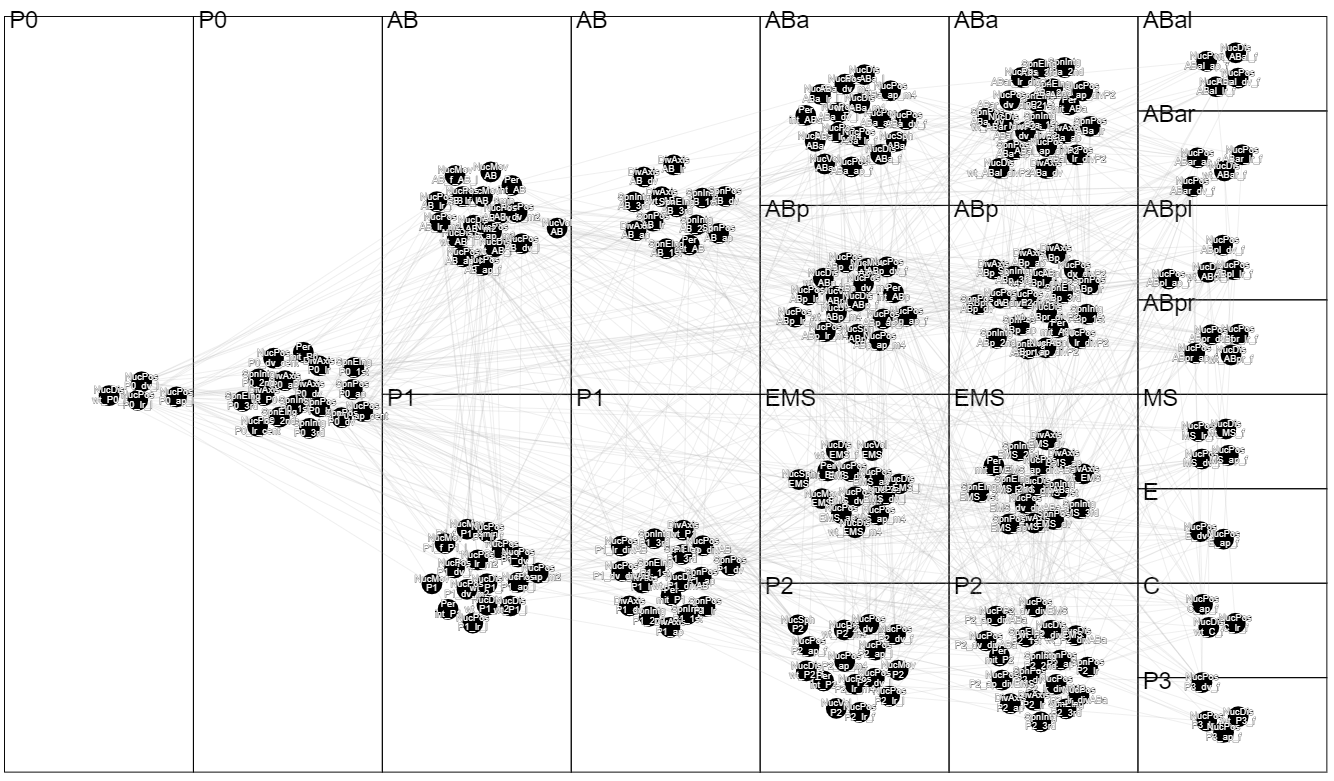
\includegraphics[width=15cm]{./images/PhenotypeNet.png}
  \caption{表現型特徴ネットワークの例}
\end{figure}

\begin{figure}
  \centering
  \label{fig:example_GIB}
  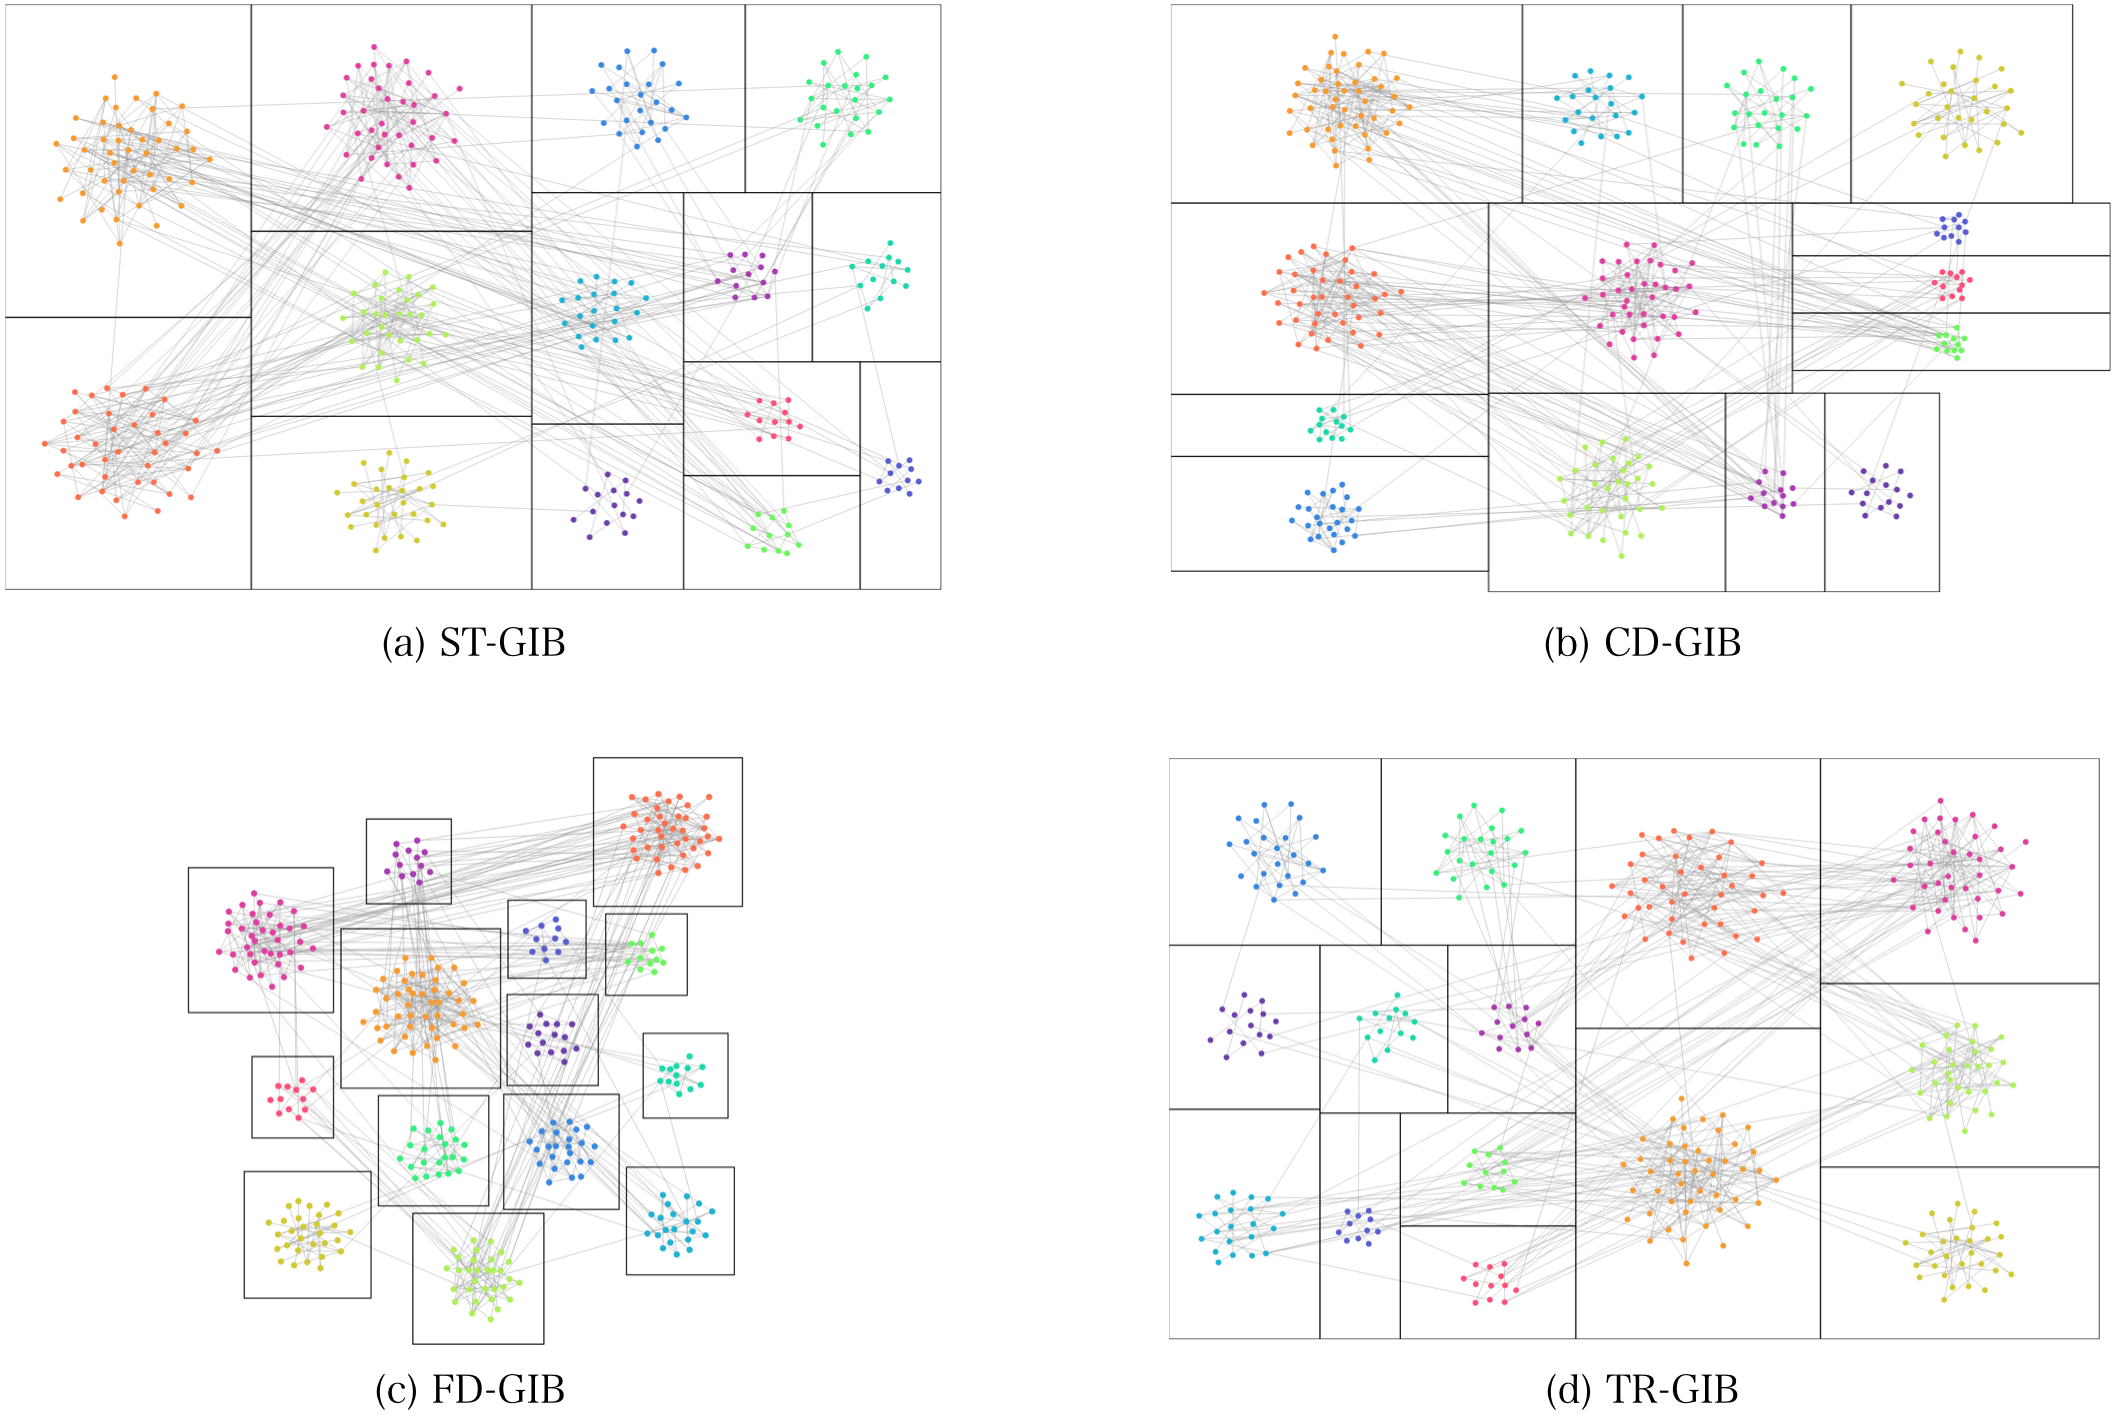
\includegraphics[width=15cm]{./images/examples.png}
  \caption{GIBレイアウトの種類。(a)ST-GIB, (b)CD-GIB, (c)FD-GIB, (d)TR-GIB}
\end{figure}


\chapter{関連研究}
\label{chap:relatedwork}

本章では関連研究について記述する。
本研究は生物学やグラフ描画、可視化の評価など様々な研究が関連するため、3節に分けてこれを述べる。
\ref{sec:vis_bio}節では生物学データの可視化について述べる。
特に、本研究は表現型特徴ネットワークの可視化に焦点を当てており、現在までの研究とその問題点について論述する。
\ref{sec:graph_for_group_structure}節ではグループ構造を持つネットワークの可視化手法について述べる。
こうした可視化手法にはいくつか種類があるが、その中でのGIBの立ち位置と、なぜGIBを研究対象にしたかを詳細に説明する。
\ref{sec:evaluation_with_eyetracking}節では視線追跡グシステムを用いた可視化の評価研究について記述する。
可視化の評価という分野は近年その重要性を高めているが、その中でも視線追跡システムを用いたものは結果をより定量的に述べられる上更なる考察を与えられるがために学術的な価値が高い。
一方で、高性能な視線追跡システムが一般に使用されるようになってから日が浅く、そのデータの膨大さから解析方法もあまり整っていない。
関連研究を詳細に述べることで、本研究の目的に即した視線データ解析を目指す。

\section{生物学データの可視化}
\label{sec:vis_bio}
顕微鏡により計測された細胞の動態を自動的に計測するバイオインメージ・インフォマティクス技術の発達により、大量の生命科学データが記録されている。
こうしたデータを解析するために、ImageJ\cite{schneider2012nih}に代表されるような取得された画像データを定量化し可視化する汎用的なツールも盛んに開発されている\cite{schindelin2012fiji,carpenter2006cellprofiler,Chen491035}

\section{Graph-drawing Method for Group Structure}
\label{sec:graph_for_group_structure}
データの重要性が広く認知されている近年では、頻繁なデータ収集や計測機器の進化によりネットワークデータはその量も複雑性も増している。
ネットワークの膨大さと複雑さに対応するため、グラフ描画の分野では様々な手法が提案されてきた。
Eadesらはforce-directed layoutと呼ばれる手法を提案した\cite{eades84}。
この手法では、ノード間の斥力とエッジ間の引力によって各ノードが配置される。
エッジが引力を持つことから、エッジにより繋がるノード同士が近くに配置され、エッジの長さが短くなる。
その計算的指標の優位性と見た目の美しさから、force-directedレイアウトは広く利用されいて\cite{Kobourov2013ForceDirectedDA}、かつこの手法にはにはいくつかの計算アルゴリズムが存在する\cite{harel2000fast,koren2003drawing,hachul2004drawing}。

一方で、グループ構造を持つ複雑ネットワークの可視化には専用に設計された可視化手法を用いるという動向がある。
大規模なネットワークデータでは、コミュニテイ検出の重要性は周知である。
複雑ネットワークの可視化にはいくつかの手法があるが、その多くはforce-directedレイアウトに基づいたものである。
グループ構造を表現する最も典型的な方法はノードを属するグループによって決まる色で描くものである\cite{mcpherson2005discovering}。
また、ノードの形をグループによって変化させるという方法も考えられる。
しかし、こうした方法は大規模な実際のデータでは効果的でないと知られている。

Vehlowらは複雑ネットワークの可視化手法に関する調査論文を発表している\cite{Vehlow2017VisualizingGS}.
彼女らは可視化手法自体とユーザー実験で用いられたタスクについて詳細に記述し、それぞれをいくつかのカテゴリに分類している。
可視化手法の分類は可視化手法とデータの構造の特徴により決まる。
前者はグループ構造が視覚的にどう表現されているかを表しており、その表現の仕方によってノード属性、並置、上書き、埋め込みという4つの分類に分けられる。
後者はグループの重複性とグループ間の階層構造性が基準となる。
ノードは同時に複数のグループに属することもあり、これの有無がグループの重複性となる。
ある2つのグループの中に包含関係があることもあり、これの有無が階層構造性となる。
Vehlowらは今までに提案された複雑ネットワーク向けの可視化手法のそれぞれのカテゴリに分けて紹介している。


% The GIB layout is also a visualization for group structure; it is presented in~\cite{rodrigues2011group,chaturvedi2014group,onoue2017optimal}.
% % There are 4 major variants of GIB, which we consider in this research: ST-GIB, CD-GIB, FD-GIB, and TR-GIB.
% % This layout has the advantage of visualizing each group in a clearly separate way, which allows the observation of the relationship between two nodes in the same group easily.
% % It can also show a group size visually with the area of a rectangular.
% This method is categorized as a superimposed visualization and is best for networks without group overlapping in Vehlow's taxonomy. ST-GIB and TR-GIB can be also applied for networks with hierarchical structure.
% % An example of network data in which GIB is effective is Twitter data with some groups defined with the user locations because their locations cannot overlap.
% Chaturvedi et al.~\cite{chaturvedi2014group} compared three types of GIBs: ST-GIB, CD-GIB, and FD-GIB, by calculating several objective measures: edge-box overlap, percent screen space wasted, execution time, and mean group-box aspect ratio.
% They also provide several case studies.
% % They observed strong differences in the computational measures among the three layouts; especially, FD-GIB is good at reducing the number of edge-box overlaps but not at saving screen space.

% Although such objective evaluation is effective, it is insufficient because certain hidden factors such as human cognition also influence readability. A user study in which participants use the graphs to complete multiple tasks could facilitate a more-thorough discussion of the layout's effectiveness and appropriately evaluate GIBs while considering such hidden factors.
% The algorithm proposed by Didimo and Montecchiani~\cite{6295786} also produces a good layout for visualizing group structure with arranging groups in boxes; however, this looks similar to FD-GIB.
% For the sake of easy comparisons, we focus on only four GIB layouts in this study.

% \subsection{アイトラッキングシステムによる可視化の評価}
% \label{sec:evaluation_with_eyetracking}
% Several studies have evaluated visualization techniques through eye tracking~\cite{burch2011evaluation,pohl2009comparing,netzel2014comparative,jianu2014display,7539393}, which have been widely used to collect gaze data and measure the participants' visual attention~\cite{andrienko2012visual,duchowski2007eye,kurzhals2014evaluating}.
% Such systems are often used to analyze how well participants perform in a user study. Researchers can elicit clues about why one visualization is better than another by analyzing gaze data.

% Burch et al.\ evaluated three variants of tree diagrams through eye tracking~\cite{burch2011evaluation}.
% %They gave participants a task to find the least common ancestor of a set of given nodes. They collected gaze data as well as task accuracy and completion time, and they analyzed it using techniques designed for the analysis of gaze data, such as trajectory map, heat map, and gaze flow between a pair of areas of interest (AOIs).
% Their analysis of eye-tracking data explained why the task-completion results differed, as they found that the task with the layout with the least accuracy required users to look over complex cross-check trajectories.

% Several studies provide guidelines on the visual analytics of eye-tracking data~\cite{andrienko2012visual,kurzhals2014evaluating,duchowski2007eye}.
% Eye-tracking datasets are often very large and difficult to analyze; hence, spatiotemporal gaze data requires specific methodologies for analysis.
% Burch et al.\ mentioned two methods for analyzing gaze data~\cite{Burch2013VisualTS}, focusing on either areas of interest (AOIs) or gaze trajectories.
% Since early studies, researchers have known that although AOI plays a crucial role in the analysis process of eye movement data, people concentrate on interesting and informative regions of a display~\cite{yarbus1967eye}.
% GIB divides the screen into boxes that are naturally regarded as AOIs. Thus, AOI analysis was also used in the present study as it is particularly in the analysis conducted herein.% For effective and meaningful analytics, it is important to know what kind of methods are most appropriate, and these studies can give researchers some hints.
% % We collect gaze data during the tasks in order to reveal which elements in a visualization affect performance.
% % We suppose that this study becomes more meaningful by following these analysis methods.

% \section{GIB Layouts}
% %{}
% This section describes the four evaluated GIB variants, examples of which are shown in Figure~\ref{GIB-examples}.
% Each graph in this figure has a different GIB layout, but all layouts are representations of the same network data.
% As regards evaluation, Chaturvedi et al.\ have performed a computational experiment on three of these layouts: ST-GIB, CD-GIB, and FD-GIB \cite{chaturvedi2014group}.
% Onoue et al.\ showed that TR-GIB is advantageous over ST-GIB in terms of computational measures \cite{onoue2017optimal}.
% Our target layouts are the four abovementioned layouts which need to be evaluated from the perspective of human cognition through user experiment.
% % We use the force-directed layout to draw network within a group, but it is also possible to use other methods.

% \subsection{ST-GIB}
% The squarified treemap GIB (ST-GIB) (Figure~\ref{GIB-examples}(a)) proposed by Rodrigues et al.~\cite{rodrigues2011group} is based on the squarified treemap algorithm developed by Bruls et al.~\cite{bruls2000squarified}.
% Bruls et al.'s method was originally designed for tree mapping, which is a visualization method that considers rectangular regions and numerical columns as inputs to divide a region into tiles, whose areas are proportional to their values~\cite{shneiderman1992tree}.

% In ST-GIB, each group is considered a vertex of the treemap and is depicted in the shape of a tile with nodes belonging to the group.
% The treemap algorithm facilitates a space-filling arrangement with boxes having low aspect ratios, which is important for analyzing the box's content~\cite{bruls2000squarified}.
% However, the ST-GIB layout exclusively uses the squarified treemap algorithm to arrange groups; hence, the relationships among nodes are not considered when drawing the tiles.
% As a result, links frequently overlap, significantly hampering the user's understanding of the network~\cite{468391,purchase1997aesthetic,purchase1998performance,purchase2002empirical}.
% To arrange tiles using ST-GIB, we utilized the squarify Python library (https://github.com/laserson/squarify) that implements Bruls' algorithm. This method arranges the boxes in order of box size, which simplifies the comparison of group sizes for users.

% \subsection{CD-GIB}
% Chaturvedi et al.~\cite{chaturvedi2014group} proposed the croissant-and-doughnut GIB (CD-GIB) (Figure~\ref{GIB-examples}(b)).
% They developed this layout to improve ST-GIB such that it considers link information connecting a node to another node belonging to a different group.
% In particular, they arranged tiles based on the G-degree and G-skewness.
% A group's G-degree is defined as the number of other groups it is connected to, and its G-skewness is the proportion of nodes included in the two most-connected groups (groups with the highest G-degree).
% A layout is then chosen from croissant-GIB, doughnut-GIB, or ST-GIB according to the total number of groups and the G-skewness of the graph.
% Chaturvedi et al.\ defined criteria for appropriately using the three methods, and we applied the same criteria.

% Croissant-GIB places the most-connected box, which has the highest G-degree, at the center-top of the screen. The other boxes are set such that they surround the most-connected box, resulting in a croissant shape. Another layout, called doughnut-GIB, assigns the most-connected box to the center with other boxes surrounding it to form a doughnut shape.

% The most-connected group is placed close to the center to reduce edge overlaps; hence, the readability is better than that when using ST-GIB.
% However, the aspect ratios of the boxes tend to be less uniform, which makes the area of the boxes difficult to estimate.

% \subsection{FD-GIB}
% Chaturvedi et al.~\cite{chaturvedi2014group} also proposed the FD-GIB layout (Figure~\ref{GIB-examples}(c)).
% In FD-GIB, the group boxes are arranged with a force-directed layout run on the whole network, with the vertices for this layout representing entire groups and the edges between them representing the links between groups.
% Then, group boxes are overlaid on this initial layout.%, centered at the group's position.
% FD-GIB can cause group overlaps, which are then removed using the PRISM method~\cite{gansner2008efficient}.

% Chaturvedi et al.\ used the Harel--Koren fast multiscale layout~\cite{harel2002graph} to arrange the rectangles in FD-GIB, but we use the D3.js force simulation~\cite{Bostock:2011:DDD:2068462.2068631} because of its easy availability and good results.
% However, as reported by Chaturvedi et al.~\cite{chaturvedi2014group}, according to experimental evaluations of several layout algorithms performed by Hachul et al.~\cite{Hachul:2005:ECF:2102325.2102348,Hachul2007LargeGraphLA}, several good options are available~\cite{harel2002graph,koren2003drawing}.
% % , such as the high-dimensional embedding approach~\cite{harel2002graph} or the algebraic multi-grid method~\cite{koren2003drawing}.

% This layout clearly displays the aggregate topology, but it uses more screen space.
% The area of each group must be smaller than that of the other layouts; hence, the relationships within a single group are more difficult to observe. However, this layout can maintain a consistent aspect ratio because of which participants can easily recognize the size differences between boxes.

% \subsection{TR-GIB}
% Onoue et al.\ developed TR-GIB to minimize the weighted sum of distances between groups by reordering the sibling nodes laid out by ST-GIB~\cite{onoue2017optimal}.
% An example of this layout is shown in Figure~\ref{GIB-examples}(d).
% This method is visually similar to ST-GIB, but the tiles are reordered by solving an optimization problem to reduce the total length of the links between groups.
% As treemaps, such as ST-GIB, have a tree-like structure, vertices with the same depth in a tree can be reordered.
% The shorter edges in TR-GIB reduce the number of edge crossings, thereby improving the readability of the graph.
% % Specifically, the sum of the distances between two groups is weighted according to the number of edges between the two groups, and this sum is taken as the group proximity.
% We expect this layout to have the advantages of ST-GIB (i.e., good aspect ratio and screen efficiency) with an additional advantage of fewer edge overlaps.




%======================================================================
%   謝辞
%======================================================================
\begin{acknowledgements}

\end{acknowledgements}



%======================================================================
%   参考文献
%======================================================================
\bibliographystyle{kueethesis}
\bibliography{sample}



%======================================================================
%   付録
%======================================================================
\appendix

\end{document}
% Local Variables:
% fill-column: 70
% End:
